\subsection{Reparameterization Trick}
\begin{frame}{}
	\LARGE VAE: \textbf{Reparameterization Trick (Pathwise Derivative Estimator)}
\end{frame}

\begin{frame}{The Problem: Sampling Blocks Gradients}
\begin{itemize}
    \item The forward pass is clear: encoder outputs $\mu(x)$ and $\sigma(x)$, we \textbf{sample} $z \sim \mathcal{N}(\mu(x), \sigma^2(x))$, and the decoder reconstructs from $z$.
    \item Training needs $\partial \mathcal{L} / \partial \mu$ and $\partial \mathcal{L} / \partial \sigma$, but the gradient path runs \textbf{through the sampling node}, and ``draw a random number'' is not a differentiable operation.
    \item So the vanilla design of just predicting $\mu$ and $\sigma$ cannot be trained end-to-end by backpropagation as it stands.
    \item Score-function (REINFORCE) estimators could work around this, but their gradients are extremely noisy.
    \item The fix is to \textbf{move the randomness out of the way}: the reparameterization trick.
\end{itemize}
\end{frame}

\begin{frame}[allowframebreaks]{Reparameterization Trick}
\textbf{Problem:} Cannot backpropagate through stochastic sampling.\\[1em]

\textbf{Solution:} Reparameterize $z$ as:
\[
z = \mu + \sigma \cdot \epsilon, \quad \epsilon \sim \mathcal{N}(0, I)
\]

\textbf{Benefit:} Enables gradient-based optimization by making the sampling operation differentiable.

\framebreak

\begin{figure}
	\centering
	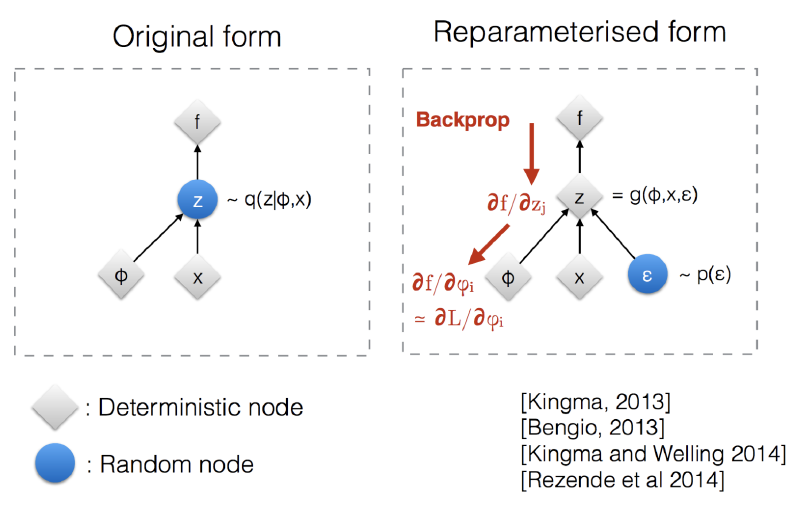
\includegraphics[height=0.8\textheight, width=\textwidth, keepaspectratio]{images/vae/reparam_trick.png}
	\caption*{Reparameterization trick to make backpropagation possible}
\end{figure}

\framebreak

\begin{figure}
	\centering
	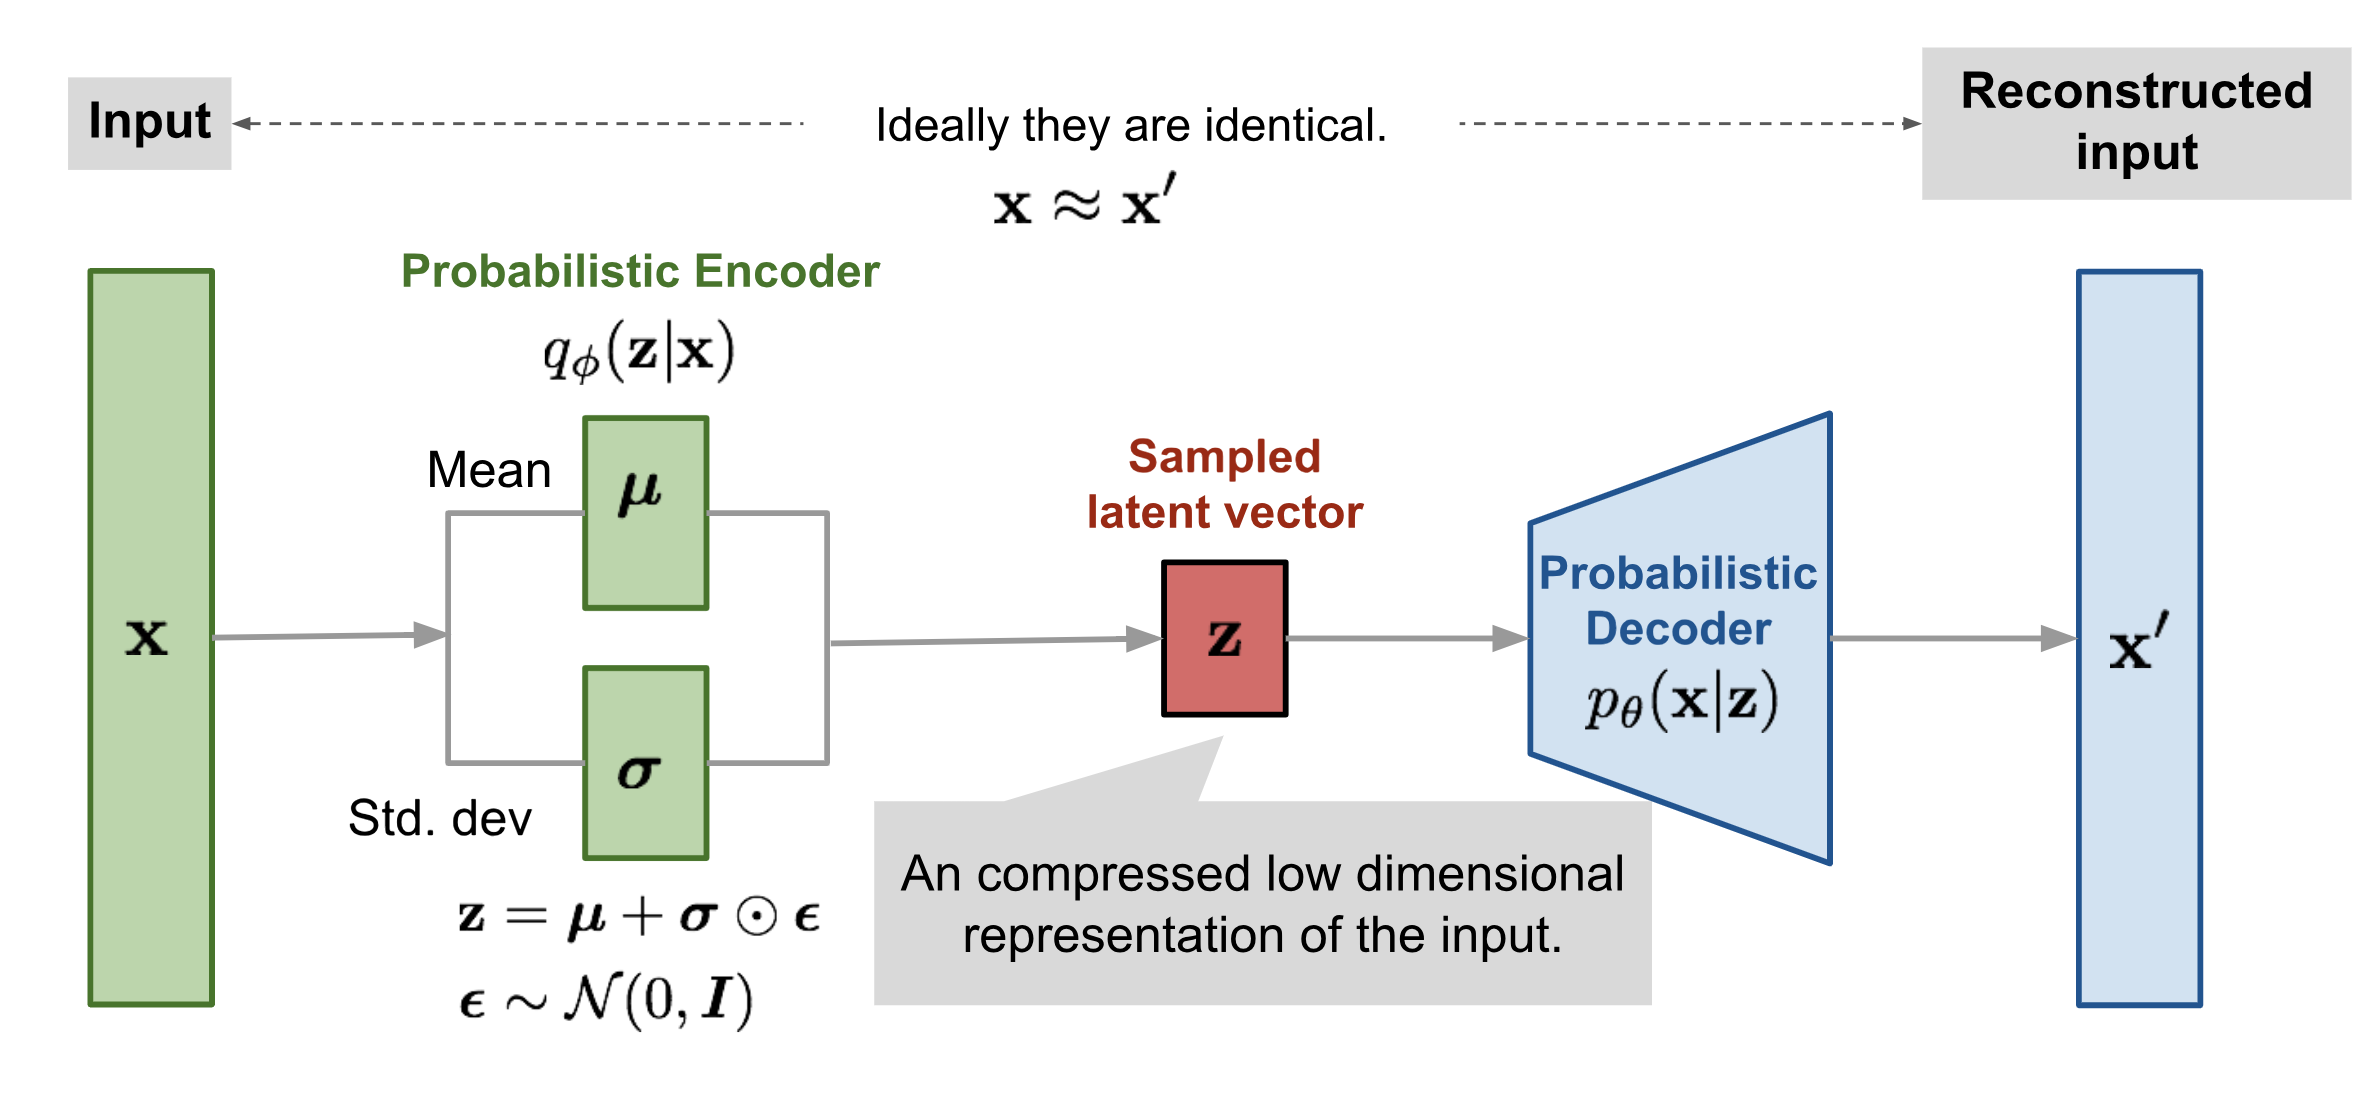
\includegraphics[height=0.8\textheight, width=\textwidth, keepaspectratio]{images/vae/reparam_trick_network.png}
	\caption*{Variational Autoencoder with reparameterization trick}
\end{figure}
\end{frame}

\begin{frame}[allowframebreaks]{Pathwise Derivative - Toy Problem}
\begin{figure}
		\centering
		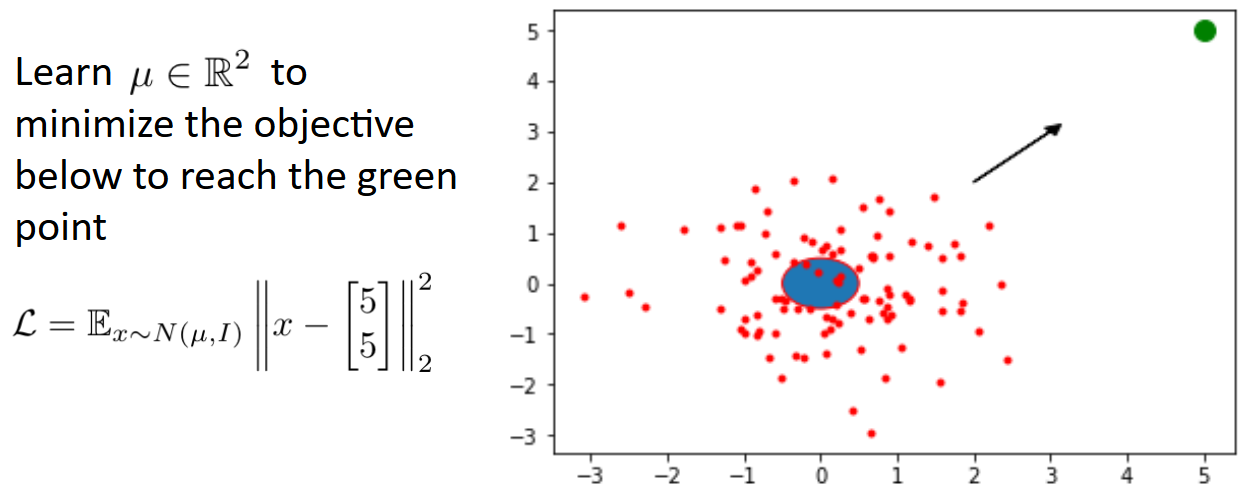
\includegraphics[height=0.9\textheight, width=\textwidth, keepaspectratio]{images/vae/toy-problem-1.png}
\end{figure}

\framebreak

\begin{figure}
		\centering
		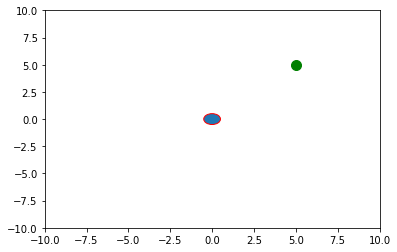
\includegraphics[height=0.8\textheight, width=\textwidth, keepaspectratio]{images/vae/toy-problem-2.png}
\end{figure}

\framebreak

\begin{figure}
		\centering
		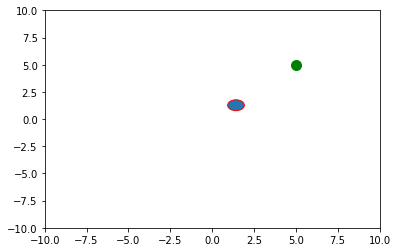
\includegraphics[height=0.8\textheight, width=\textwidth, keepaspectratio]{images/vae/toy-problem-3.png}
\end{figure}

\framebreak

\begin{figure}
		\centering
		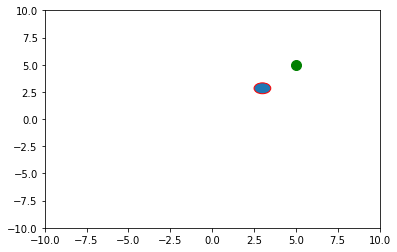
\includegraphics[height=0.8\textheight, width=\textwidth, keepaspectratio]{images/vae/toy-problem-4.png}
\end{figure}
\end{frame}